\begin{figure*}[ht]
  \centering
    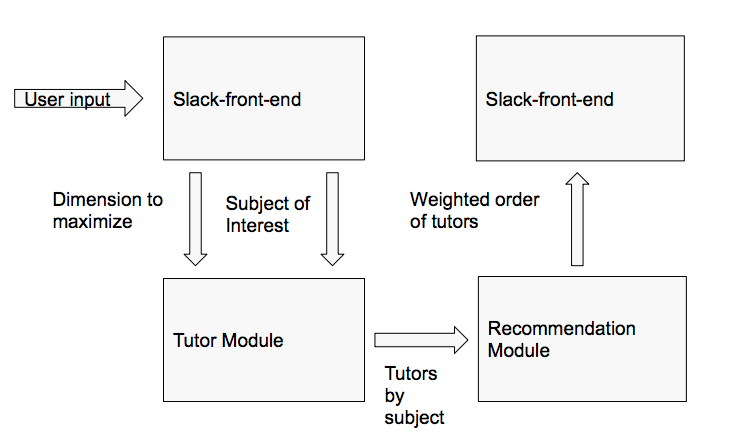
\includegraphics[width=.45\textwidth]{design_flow}
    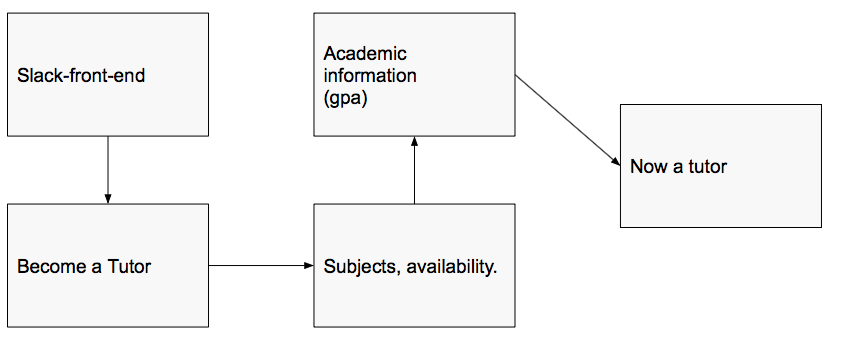
\includegraphics[width=.45\textwidth]{tutor_registration}
    % \caption{Average Levels for Frustration, Confusion, and Gaming the System per Student across their entire usage of the Tutoring System}
    \label{fig:scatterplot}
\end{figure*}
As mentioned in section \ref{sec:tutor-matching} the goal of this project is to
improve the matching done by WolfTutor.  In its original form, students input
only what subject they were interested in a tutor for and the system returned
back all students in that given subject.  While effective, this brute-force
strategy can wind up showing students an extremely large number of potential
tutors in their chat app, which can be somewhat challenging to navigate.

The original system also displayed fairly little information about the tutor
when searching.  The list of tutors returned by the ``find a tutor''
functionality contained basic information such as name and major, but did not
include information about the performance of the tutor academically or their
reviews.  To see reviews, the searching student would have to hit a ``review''
button which would then display all the reviews that tutor had at the bottom of
the screen. While this technically made the necessary information available,
this UI was challenging to use, and after getting feedback from the first round
of reviews, the team decided to make some changes to this process.  

First and foremost, however, the goal of this project is to improve the process
of chosing a tutor in WolfTutor by providing a filtered list of tutors to
students when they search for tutors in the system.  To do this, the team
identified four major metrics of a tutor to use as a basis of comparison.

\subsubsection{Overall Review Score}
The overall review score is the most obvious metric for evlauating a tutor
currently.  This score is simply a mean of the reviews (on a scale from 1 to
5) of a given tutor.  A simple average, though, has a few problems.
\begin{itemize}
\item Tutors who have used the sytem for a longer period of time are less
  sensetive to fluctuations in their rating and a dramatic change in quality
  of tutoring may not affect them appropraitely.
\item Tutors who had a temporary period of poor reviews or a single bad
  experience early in their career may struggle to find students to redeem
  their record after a small number of poor reviews.  
\end{itemize}

Given the potential for abuse, the team decided to break the reviews into a
rolling thirty day window.  By keeping reviews to the past thirty days, the
team hopes to help prevent some of the potential abuses of the mean review
score by allowing outlier reviews to fall off on a regular schedule.  This
also serves as a small optomization to the review calculation process to help
keep the calculation of the mean scores fast enough to scale in a production
system.

It is also worth noting that this window is configurable, so if a problem were
found during evaluation, this is one dimension that the system could be
tweaked to help prevent abuse.

\subsubsection{Individual Review Score}
The individual review score is one dimension that offers personalization to
the reviews.  While it is obviously a good idea to order tutors on the basis
of their overall review rating, it is also possible that particular tutors
work well with particular students.  To that end, any system making
personalized recomendations should take into account the searching student's
preferences and past experience.  This is what the individual review score
attribute attempts to do.  This score is the mean review that the current
student has given to each tutor.  

\subsubsection{Tutor score (working title)} % TODO: name this better
% TODO: what problems does this solve?  Doesn't quite make sense.

The tutor score is similar to the individual review score.  Like the
individual review score, it is a score specific to the logged in student, but
instead of being the mean review score the current student has given a given
tutor, it is the mean review score a given tutor has given to the current
user.  This attempts to solve two problems.

\begin{itemize}
\item It helps new tutors rise in the rankings.
  It helps tutors with short review history but strong experience being
  tutored show up in recommendations.
\item It helps further personalize recommendations.
\end{itemize}

\subsubsection{GPA}
The student's GPA is the last dimension the team found time to add, and it
needs little introduction.  At some universties such as Marshall University,
students are not authorized as peer tutors unless they have attained a GPA
better than some threshold.  While WolfTutor does not currently employ such a
GPA filter, it is thought that such a minimum viable threshold would probably
reveal itself in whatever culture the application was deployed to.  


%%% Local Variables:
%%% mode: latex
%%% TeX-master: "../main"
%%% End:
